\chapter[Metodologia]{Metodologia}

Esse capítulo aborda diversos tipos de metodologias e procedimentos de pesquisa, incluindo a que será utilizada durante o desenvolvimento da pesquisa deste trabalho. O capítulo está organizado em seções. Na seção 5.1, é explanado sobre as classificações de pesquisa quanto a abordagem, objetivo e procedimentos técnicos. Em seguida, na seção 5.2, é relatado o planejamento da metodologia aplicada tanto para pesquisa quanto para o desenvolvimento do software, bem como o fluxo de atividades e cronogramas.

 \section{Classificações de Metodologias de Pesquisa}
  
Pesquisar pode ser entendido como uma realização concreta de uma investigação planejada, desenvolvida e redigida de acordo com as normas da metodologia consagradas pela ciência, ou, de forma mais simples, como uma atividade para solucionar problemas \cite{kauark2010} \cite{ruiz1996}. Considerando a forma de abordagem do problema, as pesquisas são categorizadas em pesquisa quantitativa e pesquisa qualitativa. A primeira refere-se a pesquisas que podem ser quantificáveis, ou seja, é possível ser traduzida em números e requer uso de técnicas estatísticas para sua análise. A pesquisa qualitativa é descritiva, sendo assim, não pode ser analisada de forma mensurável e sim indutivamente \cite{kauark2010}.

 \par
  \indent Utilizando objetivo geral como critério de classificação, pode-se categorizar as pesquisas em três grupos: exploratória, descritiva e explicativa. A pesquisa exploratória busca obter maior conhecimento sobre um assunto específico ainda pouco conhecido tornando-o mais explícito e orientando a formulação de hipóteses \cite{gil2002}. Geralmente é realizada em forma de estudo de caso ou pesquisa bibliográfica \cite{rodrigues2007} e, para sua execução, costuma-se fazer uso de entrevistas com pessoas experientes no assunto, levantamento bibliográfico e análise de exemplos relacionados com a temática \cite{gil2002}. 

 \par
  \indent A pesquisa descritiva propõe ao investigador descrever as características de uma população ou fenômeno, ou determinar a existência de relações de dependência entre variáveis \cite{gil2002}.  Em geral, é realizada com auxílio de coleta de dados por meio de questionários e observações sistemáticas \cite{tafner2007}. Para uma correta interpretação da pesquisa, é importante que o investigador observe, registre, analise e classifique os dados de forma que não haja interferências com os fatos observados \cite{rodrigues2007}. 

 \par
  \indent O terceiro grupo refere-se à pesquisa explicativa. Essa tem como objetivo explanar sobre os fatores que determinam ou contribuem com  a ocorrência de um fenômeno específico. Essa categoria de pesquisa visa compreender os motivos de um fenômeno, enquanto a exploratória e descritiva motivam-se a entender o fenômeno em si e detalhá-lo \cite{gil2002}. Comumente é realizada por meio de pesquisa  \textit{ex-post facto} e pesquisa experimental \cite{tafner2007}.

 \par
 \indent Embora a classificação quanto ao objetivo proporcione uma visão conceitual da pesquisa, existe a necessidade de obter uma visão a nível operativo \cite{gil2002}. Nesse sentido, pode-se categorizar pesquisas quanto ao procedimento técnico utilizado. Entre eles temos:
 
\begin{description}
\item[Pesquisa Bibliográfica:] é realizada a partir do levantamento de referências teóricas sobre o tema. De forma geral, toda pesquisa inicia-se como uma pesquisa bibliográfica, mas há aquelas que dependem exclusivamente desse tipo de pesquisa. Em essência, a conclusão desse tipo de pesquisa é uma compilação das publicações referentes ao tema \cite{prodanov2013}.  

\item[Pesquisa Documental:] semelhante à pesquisa bibliográfica, diferencia-se pela natureza das fontes. Tem como base documentos sem tratamento analítico, como tabelas, cartas fotos, pinturas, dentre outros \cite{gil2002}. 

\item[Pesquisa Experimental:] seleciona grupos de assuntos coincidentes e submete-os a tratamentos diferentes. Com isso, ocorre uma verificação se há variáveis estranhas e é avaliado se as diferenças observadas nas respostas são estatisticamente significantes \cite{tafner2007}.

\item[Pesquisa \textit{ex-post facto}:] investiga possíveis relações de causa e efeito entre um determinado fato identificado pelo pesquisador e um fenômeno que ocorre posteriormente. A principal característica da pesquisa \textit{ex-post facto} é o fato de os dados serem coletados após a ocorrência dos eventos \cite{gil2002}.

\item[Levantamento (\textit{survey}):] utilizada em estudos exploratórios e descritivos, o levantamento pode ser de dois tipos: levantamento de uma amostra ou levantamento de uma população (também designado de censo). A coleta de dados realiza-se em ambos os casos por meio de questionários ou entrevistas. Em seguida, é realizada análise quantitativa dos dados e formuladas as possíveis conclusões \cite{prodanov2013}.

\item[Estudo de coorte:] diz respeito a um tipo de pesquisa em que seleciona um grupo de pessoas com uma característica comum. A partir de então, o grupo é acompanhado a fim de observar e analisar o que ocorre com elas num determinado tempo. Esse tipo de estudo pode ser categorizado em dois tipos: estudo retrospectivo e estudo prospectivo. O primeiro ocorre com a análise de dados históricos, enquanto o segundo refere-se a uma análise com dados atuais \cite{gil2002}.   

\item[Estudo de caso:] pode ser caracterizado de acordo com o estudo profundo de uma entidade bem definida como um programa, uma instituição, um sistema educativo, uma pessoa ou uma unidade social. Visa conhecer em profundidade o seu "como" e os seus "porquês", evidenciando a sua unidade e identidade própria \cite{prodanov2013}. 

\item[Estudo de campo:] similar ao levantamento, entretanto o estudo de campo busca maior aprofundamento nas questões propostas. O pesquisador deve ser imerso na comunidade a ser estudada de forma a obter maior conhecimento sobre as regras que regem o grupo. Esse tipo de estudo pode ser realizado com observação direta das atividades, entrevistas e análise de documentos, fotografias e filmagens \cite{tafner2007}.

\item[Pesquisa-ação:] esse tipo de pesquisa é ciclíca e pressupõe uma participação planejada do pesquisador na situação problemática a ser investigada. Recorre a uma metodologia sistemática, no sentido de transformar as realidades observadas, a partir da sua compreensão, conhecimento e compromisso para a ação dos elementos envolvidos na pesquisa\cite{thiollent2009}. Embora seja considerada flexível para alguns autores, outros definem as fases planejar, agir, monitorar e avaliar como etapas da execução de uma pesquisa-ação \cite{ferreira2011}. 

\item[Pesquisa participante:] similar à pesquisa-ação, difere-se quanto ao planejamento da ação. Enquanto a pesquisa-ação requer um planejamento anterior à ação do pesquisador, a pesquisa participante não pressupõe essa atividade. Com a finalidade de adquirir maior compreensão do grupo, o investigador participa da comunidade e suas atividades. A finalidade do estudo e a identidade do investigador devem ser de ciência para todos os envolvidos \cite{tafner2007}.
\end{description}

 \section{Planejamento da Metodologia Aplicada}
  
Utilizando o estudo descrito anteriormente como base, foi definida a metodologia de pesquisa que será utilizada durante o desenvolvimento do trabalho de conclusão de curso.  Foi definida também uma adaptação de metodologia para o desenvolvimento do \textit{framework}, embasada em práticas do Scrum \cite{scrum2014} e do eXtreme Programming \cite{wells2009}.  
  
  \subsection{Metodologia de Pesquisa} \label{Metodologia de Pesquisa}
  Tendo em vista o objetivo geral do trabalho, o desenvolvimento de um \textit{framework} para a geração de testes unitários, observa-se que o modelo de pesquisa que mais se enquadra para o contexto é um misto de pesquisa exploratória, na medida em que se busca criar maior familiaridade com a temática, e pesquisa experimental, pois se pretende criar condições em ambiente controlado para averiguar determinados casos, com afinalidade de testar o \textit{framework}. A abordagem da pesquisa será quantitativa e qualitativa. Haverá análise dos resultados de forma objetiva, como por exemplo, para cobertura de testes unitários do software alvo. Além disso, será analisado o uso das boas práticas de programação no código-fonte do \textit{framework}, o que caracteriza uma abordagem qualitativa.
  \par
  \indent Devido à necessidade da constante participação planejada dos pesquisadores, cabe ressaltar o uso da modalidade de pesquisa-ação. Isso conferirá ciclos de coleta e análise de dados e desenvolvimento para alteração do objeto de estudo, conforme as análises do ciclo anterior.

 \subsection{Metodologia de Desenvolvimento do Software} \label{Metodologia de Desenvolvimento do Software}
  No que se refere ao desenvolvimento do software, pretende-se utilizar uma adaptação do Scrum, com \textit{Sprints} de quinze dias e algumas de suas práticas, a saber: estimativas relativas, \textit{timebox}, \textit{backlog}, definição de pronto e quadro de tarefas \cite{scrum2014}. Procurar-se-á prover o desenvolvimento também com algumas práticas do eXtreme Programming, como \textit{Planning Poker}, Padronização do Código, Integração Contínua e Programação em Pares \cite{wells2009}.
 
 \subsection{Fluxo de Atividades}
 	
 	Utilizando as metodologias definidas para a execução do trabalho de conclusão de curso 01 e 02, foi estabelecido um fluxo de atividades que possibilitará o alcance dos objetivos do projeto.
 	
 \par
 \indent Inicialmente, foram realizados estudos sobre a temática escolhida. Em seguida, foram determinados o escopo do projeto e a proposta inicial resumindo os objetivos, justificativa, cronograma preliminar, entre outros aspectos introdutórios que guiaram as atividades seguintes. O estudo e a definição  da metodologia utilizada, bem como o do suporte tecnológico, ocorreram em paralelo com a pesquisa e documentação do referencial teórico base para o desenvolvimento do \textit{framework} proposto. Após essas definições, foi elaborada a primeira versão detalhada da proposta do software a ser implementado. Definiu-se também uma prova de conceito, de forma a auxiliar o refinamento da proposta. Em seguida, ocorreu a implementação da prova de conceito utilizando os ciclos de pesquisa-ação e \textit{sprints}. Com os resultados, houve a finalização da monografia com as atualizações que se fizeram necessárias. A finalização do trabalho de conclusão de curso 01 ocorrerá após a primeira apresentação para a banca avaliadora.
 \par
 \indent O trabalho de conclusão de curso 02 iniciará com as correções e refinamentos solicitados na apresentação. Em seguida,  executar-se-á o desenvolvimento do \textit{framework} proposto, utilizando pesquisa-ação e adaptação do Scrum. Será efetuada uma análise dos resultados obtidos, verificando se os objetivos estabelecidos no início do projeto foram satisfatoriamente atendidos. Por fim, será adicionado à monografia um relato do que foi executado junto com a análise de resultados.  A apresentação do trabalho de conclusão de curso 02 representará o fim do projeto.
 	
  \begin{figure}[h]
    \centering
    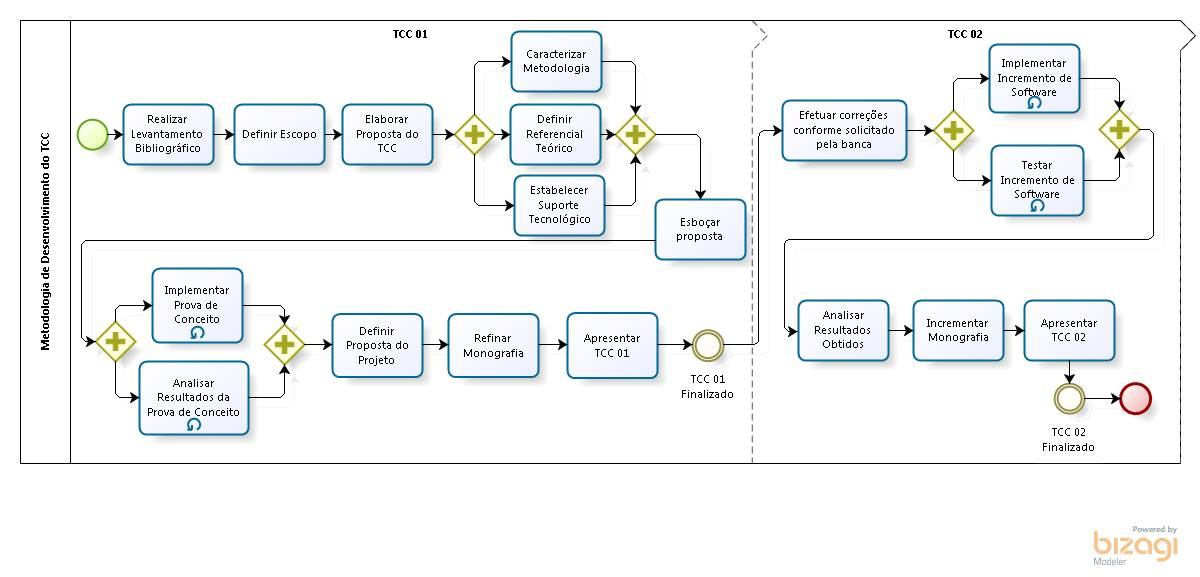
\includegraphics[width=\textwidth]{figuras/processo.jpg}
    \caption{Fluxo de Atividades do trabalho de conclusão de curso}
    \label{fig:processo}
  \end{figure}

\par 
\indent A Figura \ref{fig:processo} representa o fluxo de atividades utilizado no trabalho de conclusão de curso, como descrito anteriormente.  
  
    \begin{figure}[h]
    \centering
    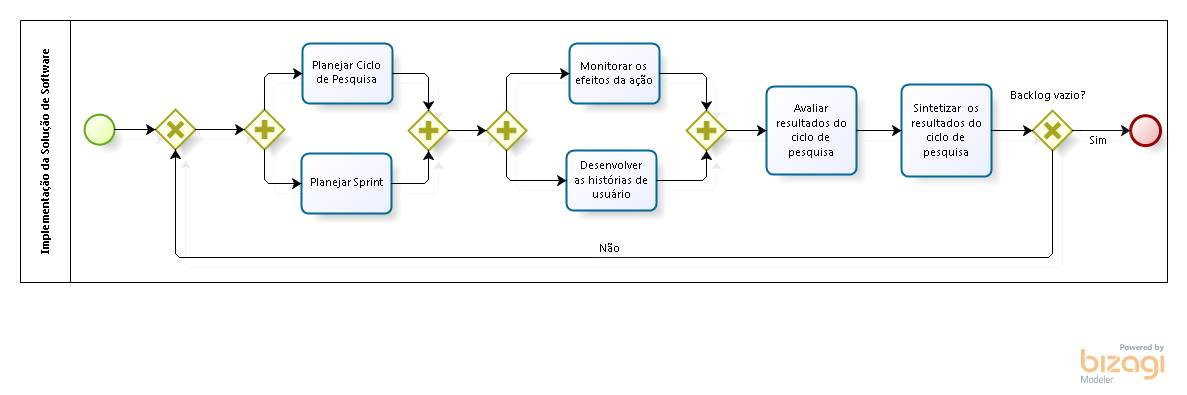
\includegraphics[width=\textwidth]{figuras/ProcessoInterno.jpg}
    \caption{Fluxo de Atividades da Implementação da Solução de Software}
    \label{fig:processointerno}
  \end{figure}

\par 
\indent A Figura \ref{fig:processointerno} demonstra a adaptação do Scrum e o uso de pesquisa-ação no desenvolvimento do \textit{framework}. 
 
 \subsection{Cronograma}
 
	Os cronogramas a seguir evidenciam o plano de execução, visão temporal, das atividades referentes ao trabalho de conclusão de curso 01 e 02. Por ser uma visão preliminar, os cronogramas podem ser alterados, caso haja necessidade. 
	  
\begin{table}[h]
  \tiny
  \centering
  \caption{Cronograma para o trabalho de conclusão de curso 1}
  \label{cronograma-tcc-1}
  \begin{tabular}{| c | c | c | c | c | c |}
    \hline
    Atividades & Agosto & Setembro & Outubro & Novembro & Dezembro \\ \hline
    Realizar Levantamento Bibliográfico & X &  &  &  &  \\
    Definir Escopo & X &  &  &  &  \\
    Elaborar Proposta Inicial do TCC & X & X &  &  &  \\
    Caracterizar Metodologia &  & X &  &  &  \\
    Definir Referencial Teórico &  & X &  &  &  \\
    Estabelecer Suporte Tecnológico &  & X &  &  &  \\
    Esboçar Proposta &  & X & X &  &  \\
    Implementar Prova de Conceito &  &  & X &  &  \\
    Analisar Resultados da Prova de Conceito &  &  & X &  &  \\
    Definir Proposta do Projeto &  &  &  & X &  \\
    Refinar Monografia &  &  &  & X &  \\
    Apresentar TCC 01 &  &  &  & X & X \\ \hline
  \end{tabular}
\end{table}
  
\begin{table}[h]
  \tiny
  \centering
  \caption{Cronograma para o trabalho de conclusão de curso 2}
  \label{cronograma-tcc-2}
  \begin{tabular}{| c | c | c | c | c | c |}
  \hline
    Atividades & Fevereiro & Março & Abril & Maio & Junho \\ \hline
    Efetuar Correções conforme solicitado pela banca & X &  &  &  &  \\
    Implementar Incremento de Software &  & X & X & X &  \\
    Testar Incremento de Software &  & X & X & X &  \\
    Analisar Resultados Obtidos &  &  & X & X &  \\
    Incrementar Monografia &  &  &  & X & X \\
    Apresentar TCC 2 &  &  &  &  & X \\ \hline
  \end{tabular}
\end{table}
  
  \section{Resumo do Capítulo}
  Este capítulo abordou sobre as metodologias de pesquisa, classicando-as em três aspectos: quanto ao objetivo, procedimentos técnicos e abordagem de pesquisa. Foi definida uma adaptação da metodologia de pesquisa-ação, bem como o fluxo de atividades e o cronograma que se adequam ao desenvolvimento deste trabalho.